\section{A trained transformer}
\label{sec:trained}

\paragraph{Setup.}
We follow the base paper's protocol as closely as its text allows.
Clips have 8 frames of $32\times32$ grayscale pixels and are cut into $8\times8$ patches, giving 128 tokens.
The background is a static Gaussian random field in six smooth modes with known variances, so that its spread in generated clips can be measured; one or two textured sprites move over it with sub-pixel motion.
On average $62\,\%$ of the 16 positions are static.
The model is a diffusion transformer~\cite{peebles2023dit} with $1.27$M parameters (4 layers, width 128, adaLN-zero conditioning, additive spatial and temporal position embeddings), trained with rectified flow~\cite{liu2023rectified} for 12k steps on a CPU and sampled with 20 Euler steps.
Speedups are analytic FLOP counts that include every draft and warm-up call; ``projected'' applies the same token counts to the base paper's 75.6k-token, 40-layer, width-3072 model.
Token removal is executed through an attention bias, which a unit test shows to be identical to physical removal.
Fidelity is the median PSNR (peak-to-peak 2) over $\AN$ noise seeds.

Every method is scored against the \emph{original} sample: 20-step full compute from the untouched noise.
We also report the base paper's own metric, the spread of the generated background coefficients relative to full compute, and the texture (mean absolute difference from a $3\times3$ blur) and motion (mean absolute frame difference) of the generated clips relative to full compute.
Static maps come from an oracle (the original sample itself), from a 2-step draft, or from the trajectory at the switch step; thresholds are set on separate seeds, to $95\,\%$ precision against the oracle, or to the best F1 (``aggressive'').
As in the base paper, the model's own samples are imperfect; they are under-dispersed (background spread $\ABgData$ of the data's) and show patch seams.

\begin{figure*}[t]
\centering
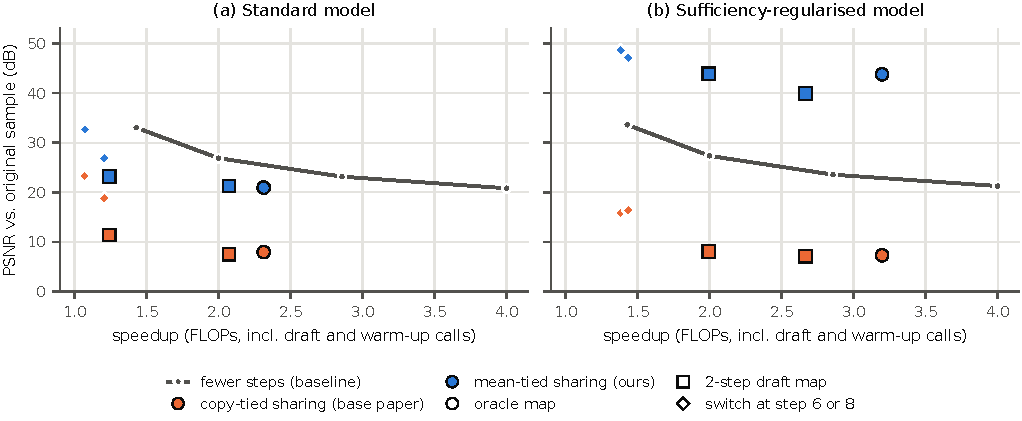
\includegraphics[width=0.93\textwidth]{../figures/fig_tradeoff.pdf}
\caption{Fidelity to the original sample against speedup, the base paper's Fig.~4 redrawn with every method scored against the same reference. (a)~Standard training: both ways of tying lie below the fewer-steps baseline; averaging is about 13\,dB above copying. (b)~After the sufficiency fine-tune: mean-tied sharing lies 15--20\,dB above the baseline; copying does not move.}
\label{fig:tradeoff}
\end{figure*}

\begin{table*}[t]
\centering
\caption{Frame sharing on equal footing with the baseline. PSNR is against the original 20-step full-compute sample from the untouched noise (median over $\AN$ seeds). ``bg'', ``tex.'' and ``mot.'': background spread, texture and motion relative to full compute (1 is correct). Left: standard training. Right: the same network after a short fine-tune with the sufficiency regulariser (Eq.~\ref{eq:reg}).}
\label{tab:main}
\small
\setlength{\tabcolsep}{3.4pt}
\begin{tabular}{@{}l rrrrrr c rrrrrr@{}}
\toprule
 & \multicolumn{6}{c}{Standard model} && \multicolumn{6}{c}{Sufficiency-regularised model}\\
\cmidrule(lr){2-7}\cmidrule(l){9-14}
Method & \makecell[r]{shared\\(\%)} & \makecell[r]{speed-\\up} & proj. & \makecell[r]{PSNR\\(dB)} & bg & \makecell[r]{tex.\,/\\mot.} && \makecell[r]{shared\\(\%)} & \makecell[r]{speed-\\up} & proj. & \makecell[r]{PSNR\\(dB)} & bg & \makecell[r]{tex.\,/\\mot.}\\
\midrule
\tabinput{generated/table_main.tex}
\bottomrule
\end{tabular}
\end{table*}

\subsection{Standard training: the base paper's result, on both footings}

Table~\ref{tab:main} (left) and Fig.~\ref{fig:tradeoff}a give the picture.

\paragraph{Copy-tied sharing reproduces the base paper.}
Against full compute from its own tied noise, copy-tied sharing scores $\ACopyOwnRef$\,dB; against the original sample it scores $\ACopyOrig$\,dB.
These are the two numbers of the base paper ($43.6$ and $11$--$15$\,dB), and only the first was put in its comparison.
The copied noise does what Theorem~\ref{thm:copy} says: the background is $\ACopyStd\times$ too dispersed, where the Gaussian law predicts $\ALawPred$ for the tied share (Fig.~\ref{fig:law}b), and the static patches fill with high-contrast texture, $\ACopyTex\times$ the normal amount (Fig.~\ref{fig:examples}).
The network has been handed noise and told it is signal.

\paragraph{Mean-tied sharing removes the over-dispersion.}
With the same map, the same token removal and the same FLOPs, averaging brings the background spread to $\AMeanStd$ and the fidelity to the original from $\ACopyOrig$ to $\AMeanOrig$\,dB.
The control that scales the leader's noise by $1/\sqrt F$ again gives the right spread ($\AColdStd$) and a different sample ($\AColdOrig$\,dB).

\paragraph{But it is not sample-preserving, and it loses to fewer steps.}
$\AMeanOrig$\,dB is far from exact.
At the same speedup, simply taking fewer steps is closer to the original sample ($\AFewerTen$\,dB at $2\times$, $\AFewerSeven$\,dB at $2.9\times$), and this holds for every map we tried (Fig.~\ref{fig:tradeoff}a).
The loss is not in the compute reuse: full compute from mean-tied noise, with no token removed, lands at the same $\AMeanFullOrig$\,dB, and sharing reproduces \emph{that} to $\AMeanOwnRef$\,dB.
It is in the network's response to tied tokens.
Mean-tied samples carry $\AMeanTex\times$ the texture and $\AMeanMot\times$ the motion of full-compute samples: the error has moved from the tied tokens into the untied ones.
So on a network trained in the standard way, the base paper's claim that frame sharing beats fewer steps does not survive an equal footing, with either way of tying the noise.

\begin{figure*}[t]
\centering
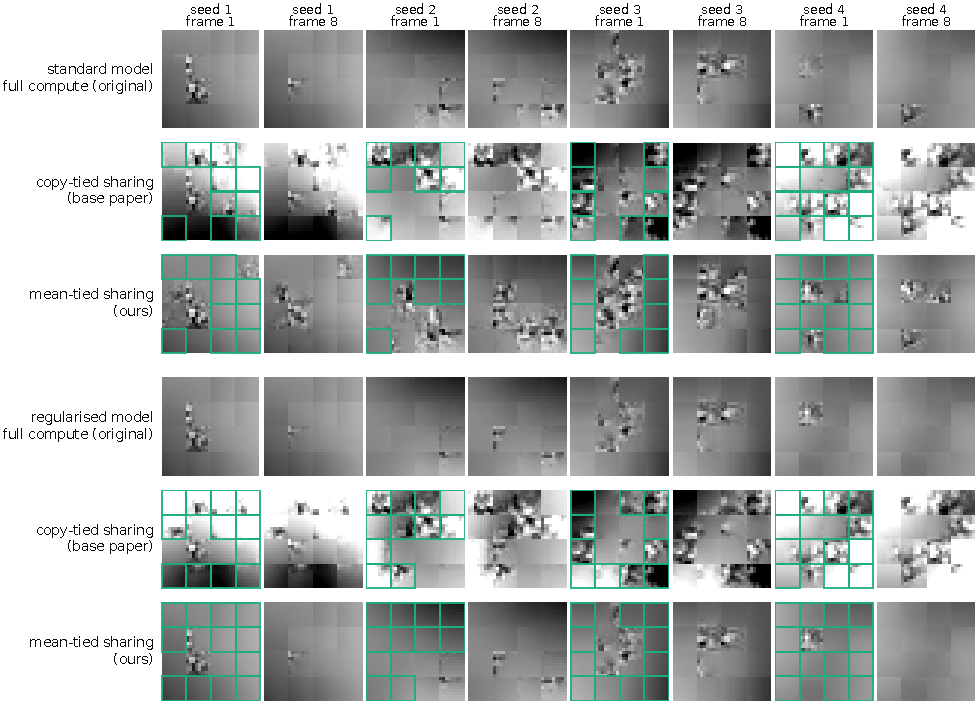
\includegraphics[width=\textwidth]{../figures/fig_examples.pdf}
\caption{Four seeds, first and last frame, oracle map (shared positions outlined in the first frame). Copy-tied sharing fills the shared patches with saturated texture on either model: noise taken for signal. Mean-tied sharing gives plausible but different clips on the standard model and reproduces the original clips on the regularised one. The regularised model's sprites are fainter, the cost discussed in \S\ref{sec:trained}.}
\label{fig:examples}
\end{figure*}

\subsection{Why: the network is not invariant to the deviations}

Lemma~\ref{lem:suff} says the ideal denoiser ignores the deviations $\delta$.
We test this directly by scaling the deviations of the static starting noise by a factor $\alpha$ and generating with full compute; an ideal denoiser returns the same sample for every $\alpha$.
The trained network does not (Table~\ref{tab:variants}): shrinking the deviations by only $10\,\%$ already moves the sample to $\VarAAlphaNine$\,dB, and removing them gives $\VarAAlphaZero$\,dB.
Its \emph{consistency error}, the mean squared difference between the frame-mean velocity on an untouched input and the velocity on the mean-tied input, is $\VarACons\times10^{-3}$ where the ideal value is zero.
Longer standard training barely changes this ($\VarSixAlphaZero$\,dB at 6k steps, $\VarAAlphaZero$\,dB at 12k, $\VarCAlphaZero$\,dB after 3k more).
A network that has only ever seen independent noise uses the deviations as a cue, most plausibly for how noisy its input is; a tied token looks too clean for its time step.

\subsection{Teaching sufficiency}

We fine-tune the standard model for 3k steps (a quarter of its training) with the regulariser of Eq.~\ref{eq:reg}, $\lambda=50$.
The consistency error falls by a factor of $\VarConsDrop$ (Table~\ref{tab:variants}), and the right half of Table~\ref{tab:main} and Fig.~\ref{fig:tradeoff}b change character.

\paragraph{Mean-tied sharing becomes sample-preserving.}
With the oracle map it shares $\BOracleStatic\,\%$ of the positions, uses $\BOracleSpeedup\times$ fewer FLOPs ($\BOracleProj\times$ projected), and reproduces the original sample at $\BMeanOrig$\,dB (10th percentile over seeds $\BMeanOrigLo$\,dB).
With the 2-step draft map of the base paper, which needs no oracle, it reaches $\BMeanDraftOrig$\,dB at $\BDraftSpeedup\times$ and, at the aggressive threshold, $\BMeanAggrOrig$\,dB at $\BAggrSpeedup\times$ ($\BDraftProj\times$ and $\BAggrProj\times$ projected), draft included; the fewer-steps baseline is at $\BFewerTen$\,dB at $2\times$ and $\BFewerSeven$\,dB at $2.9\times$.
Texture is unchanged ($\BMeanTexFine$ of full compute) and so is motion on the positions that are not shared ($\BMeanMotUnshared$); the overall motion measure is $\BMeanMotFine$ because full compute leaves a faint frame-to-frame jitter on static positions, $\BJitterShare\,\%$ of its motion, which sharing removes by construction.
Switching mid-generation, which the base paper reports as a failure, now works without any draft: collapsing to the mean at step 8 gives $\BMeanEightOrig$\,dB, where collapsing to the leader gives $\BCopyEightOrig$\,dB.
These are the fidelities the base paper reported for frame sharing, measured this time against the sample the model would have produced anyway.

\paragraph{Copying is not rescued.}
On the same network, copy-tied sharing stays at $\BCopyOrig$\,dB with backgrounds $\BCopyStd\times$ too dispersed.
The regulariser makes the network a better approximation of the ideal denoiser; it cannot make a single noise sample look like the mean of eight.

\paragraph{Proportional attention matters, and is not exact.}
Without the $\log F$ bias, mean-tied sharing falls to $\BPlainOrig$\,dB.
With it, one forward call on tied tokens differs from full attention by $\APropTrained\,\%$ in the standard model against $\APlainTrained\,\%$ without it: a large gain, as the base paper found, and not an identity (Table~\ref{tab:errata}, item~11).

\subsection{What the regulariser costs}

The regulariser changes the generator.
Table~\ref{tab:variants} compares full-compute samples of each model variant with the training data.
Continuing standard training for the same 3k steps changes nothing: the consistency error stays at $\VarCCons\times10^{-3}$, mean-tying at $\VarCAlphaZero$\,dB, texture and motion as before.
The effect of the fine-tune is the regulariser's, not that of more training.

Its price is texture.
With $\lambda=50$, full-compute samples carry $\VarBTex$ of the data's texture where the standard model carries $\VarATex$, and the regression loss on untouched inputs is $\VarBFitRise\,\%$ higher than the control's.
The sprites are fainter (Fig.~\ref{fig:examples}); more positions are static, which is part of why the regularised model shares more.
In motion the two models err in opposite directions: the standard one moves too much ($\VarAMot$ of the data's frame difference) and the regularised one too little ($\VarBMot$).
Background spread is unchanged.

A gentler setting keeps most of the benefit.
With $\lambda=5$ the consistency error still falls $\VarFiveConsDrop$-fold, mean-tying reaches $\VarFiveAlphaZero$\,dB, the regression loss is within $\VarFiveFitRise\,\%$ of the control's, texture drops less ($\VarFiveTex$) and motion moves towards the data ($\VarFiveMot$).
On that model, mean-tied sharing with the 2-step draft map reproduces the original sample at $\WDraftOrig$\,dB with $\WDraftSpeedup\times$ fewer FLOPs ($\WAggrOrig$\,dB at $\WAggrSpeedup\times$ with the aggressive threshold; fewer steps: $\WFewerTen$ and $\WFewerSeven$\,dB at $2\times$ and $2.9\times$), and copying stays at $\WCopyOrig$\,dB.
We tried only these two weights.
We suspect the network buys part of its invariance by leaning less on its noisy input, which is the cheapest way to ignore the deviations and also blurs the sprites; the ideal denoiser shows that this is not necessary, so longer training or a better-placed weight may remove the cost.
That is open.

\begin{table}[t]
\centering
\caption{Model variants. ``Cons.'': consistency error $\times10^{3}$ (0 for an ideal denoiser). ``$\alpha{=}0.9$'' and ``mean'': PSNR against the original sample after scaling the frame deviations of the static starting noise by $0.9$ and by $0$ (full compute, oracle map); ``copy'': after copying the leader's noise. Last three columns: texture, motion and background spread of full-compute samples relative to the training data.}
\label{tab:variants}
\small
\setlength{\tabcolsep}{2.6pt}
\begin{tabular}{@{}l r rrr rrr@{}}
\toprule
 & & \multicolumn{3}{c}{PSNR vs.\ original (dB)} & \multicolumn{3}{c}{vs.\ data}\\
\cmidrule(lr){3-5}\cmidrule(l){6-8}
Model & Cons. & $\alpha{=}0.9$ & mean & copy & tex. & mot. & bg\\
\midrule
\tabinput{generated/table_variants.tex}
\bottomrule
\end{tabular}
\end{table}

\subsection{Distribution test}

Per-sample fidelity cannot say whether an accelerated sampler still draws from the model's distribution when it does not reproduce the sample.
We train a small 3D CNN to tell 2{,}048 accelerated samples from 2{,}048 full-compute samples on fresh seeds (classifier two-sample test~\cite{lopezpaz2017c2st}; 0.5 means indistinguishable; white noise of standard deviation 0.03 is added to both sides so that the faint jitter full compute leaves on static positions is not a cue).
On the standard model (Table~\ref{tab:c2st}), copy-tied sharing is the most detectable sampler we tested ($\ACtCopy$) although it saves the least.
Mean-tied sharing is less detectable ($\ACtMean$) but no better than 7-step sampling ($\ACtFewerSeven$): the texture excess of Table~\ref{tab:main} is a real shift of the distribution.
On the regularised model the classifier cannot tell mean-tied sharing from full compute ($\BCtMean$, control $\BCtControl$), while copy-tied sharing ($\BCtCopy$) and fewer steps ($\BCtFewerTen$, $\BCtFewerSeven$) remain detectable.

\begin{table}[t]
\centering
\caption{Classifier two-sample test against 20-step full compute of the same model (held-out accuracy, mean of 3 classifier seeds; 0.5 is indistinguishable).}
\label{tab:c2st}
\small
\begin{tabular}{@{}l rr@{}}
\toprule
Sampler & Standard & Regularised\\
\midrule
\tabinput{generated/table_c2st.tex}
\bottomrule
\end{tabular}
\end{table}

\subsection{Two further checks}

\paragraph{Static tokens settle earlier, roughly as predicted.}
In full-compute runs of the standard model, the clean prediction of a moving token comes within $0.05$ RMS of its final value at step $\ASettleMoving$ of 20 (median), that of a static token at step $\ASettleStatic$.
Eq.~\ref{eq:clock} maps step $\ASettleMoving$ to step $\ASettlePred$ for $F=8$.
The base paper measured 7 and 4.
Static content is also simpler, so this is consistent with the clock rather than a test of it.

\paragraph{FLOPs and time.}
The FLOP model is not a measurement, so we timed the standard model on a CPU with the shortened sequences built physically (batch 32, 4 threads).
With 8, 12 and 16 of 16 positions shared, the forward pass is $\WallEight\times$, $\WallTwelve\times$ and $\WallSixteen\times$ faster, where the FLOP model says $\FlopEight\times$, $\FlopTwelve\times$ and $\FlopSixteen\times$.
So at this size the count is a fair guide.
It says little about a large model on a GPU, where attention dominates and memory traffic matters.



